\SourceLeaf{359}

Es erscheint also ein $\alpha+\beta.i$ wie $\alpha+\dfrac{\beta z' - \alpha\cdot x\sin\lambda}{z}\cdot i$ oder die beiden Radien des Kreises $1$ und $i$ in der ersten Projection erscheinen als conjugirte Halbmesser der Ellipse in der zweiten Projection $1-\dfrac{x\sin\lambda}{z}\cdot i$ und $\dfrac{z'}{z}\cdot i$, woraus sich nach p.\,164 [des Handbuches\HistoricalNote{*)}{[*)}{Dieser Band, S.\,339.]} die Dimensionen der Projectionsellipse leicht ableiten lassen.



\Needspace{20\baselineskip}
\begin{center}
[II.]
\end{center}

\begin{center}
\bfseries [STEREOGRAPHISCHE UND CENTRALE PROJECTION.]
\end{center}

\begin{center}
[1.]
\end{center}

\begin{center}
Zusammenhang der stereographischen und der Centralprojection, so dass\\
Massstab für jene im Pol $C$ halb so gross als für diese.
\end{center}

Der Kreis durch $AB$ stellt für erstere den Äquator, für letztere den Parallel von $45^0$ vor.

\begin{center}\resizebox{4.0cm}{!}{%
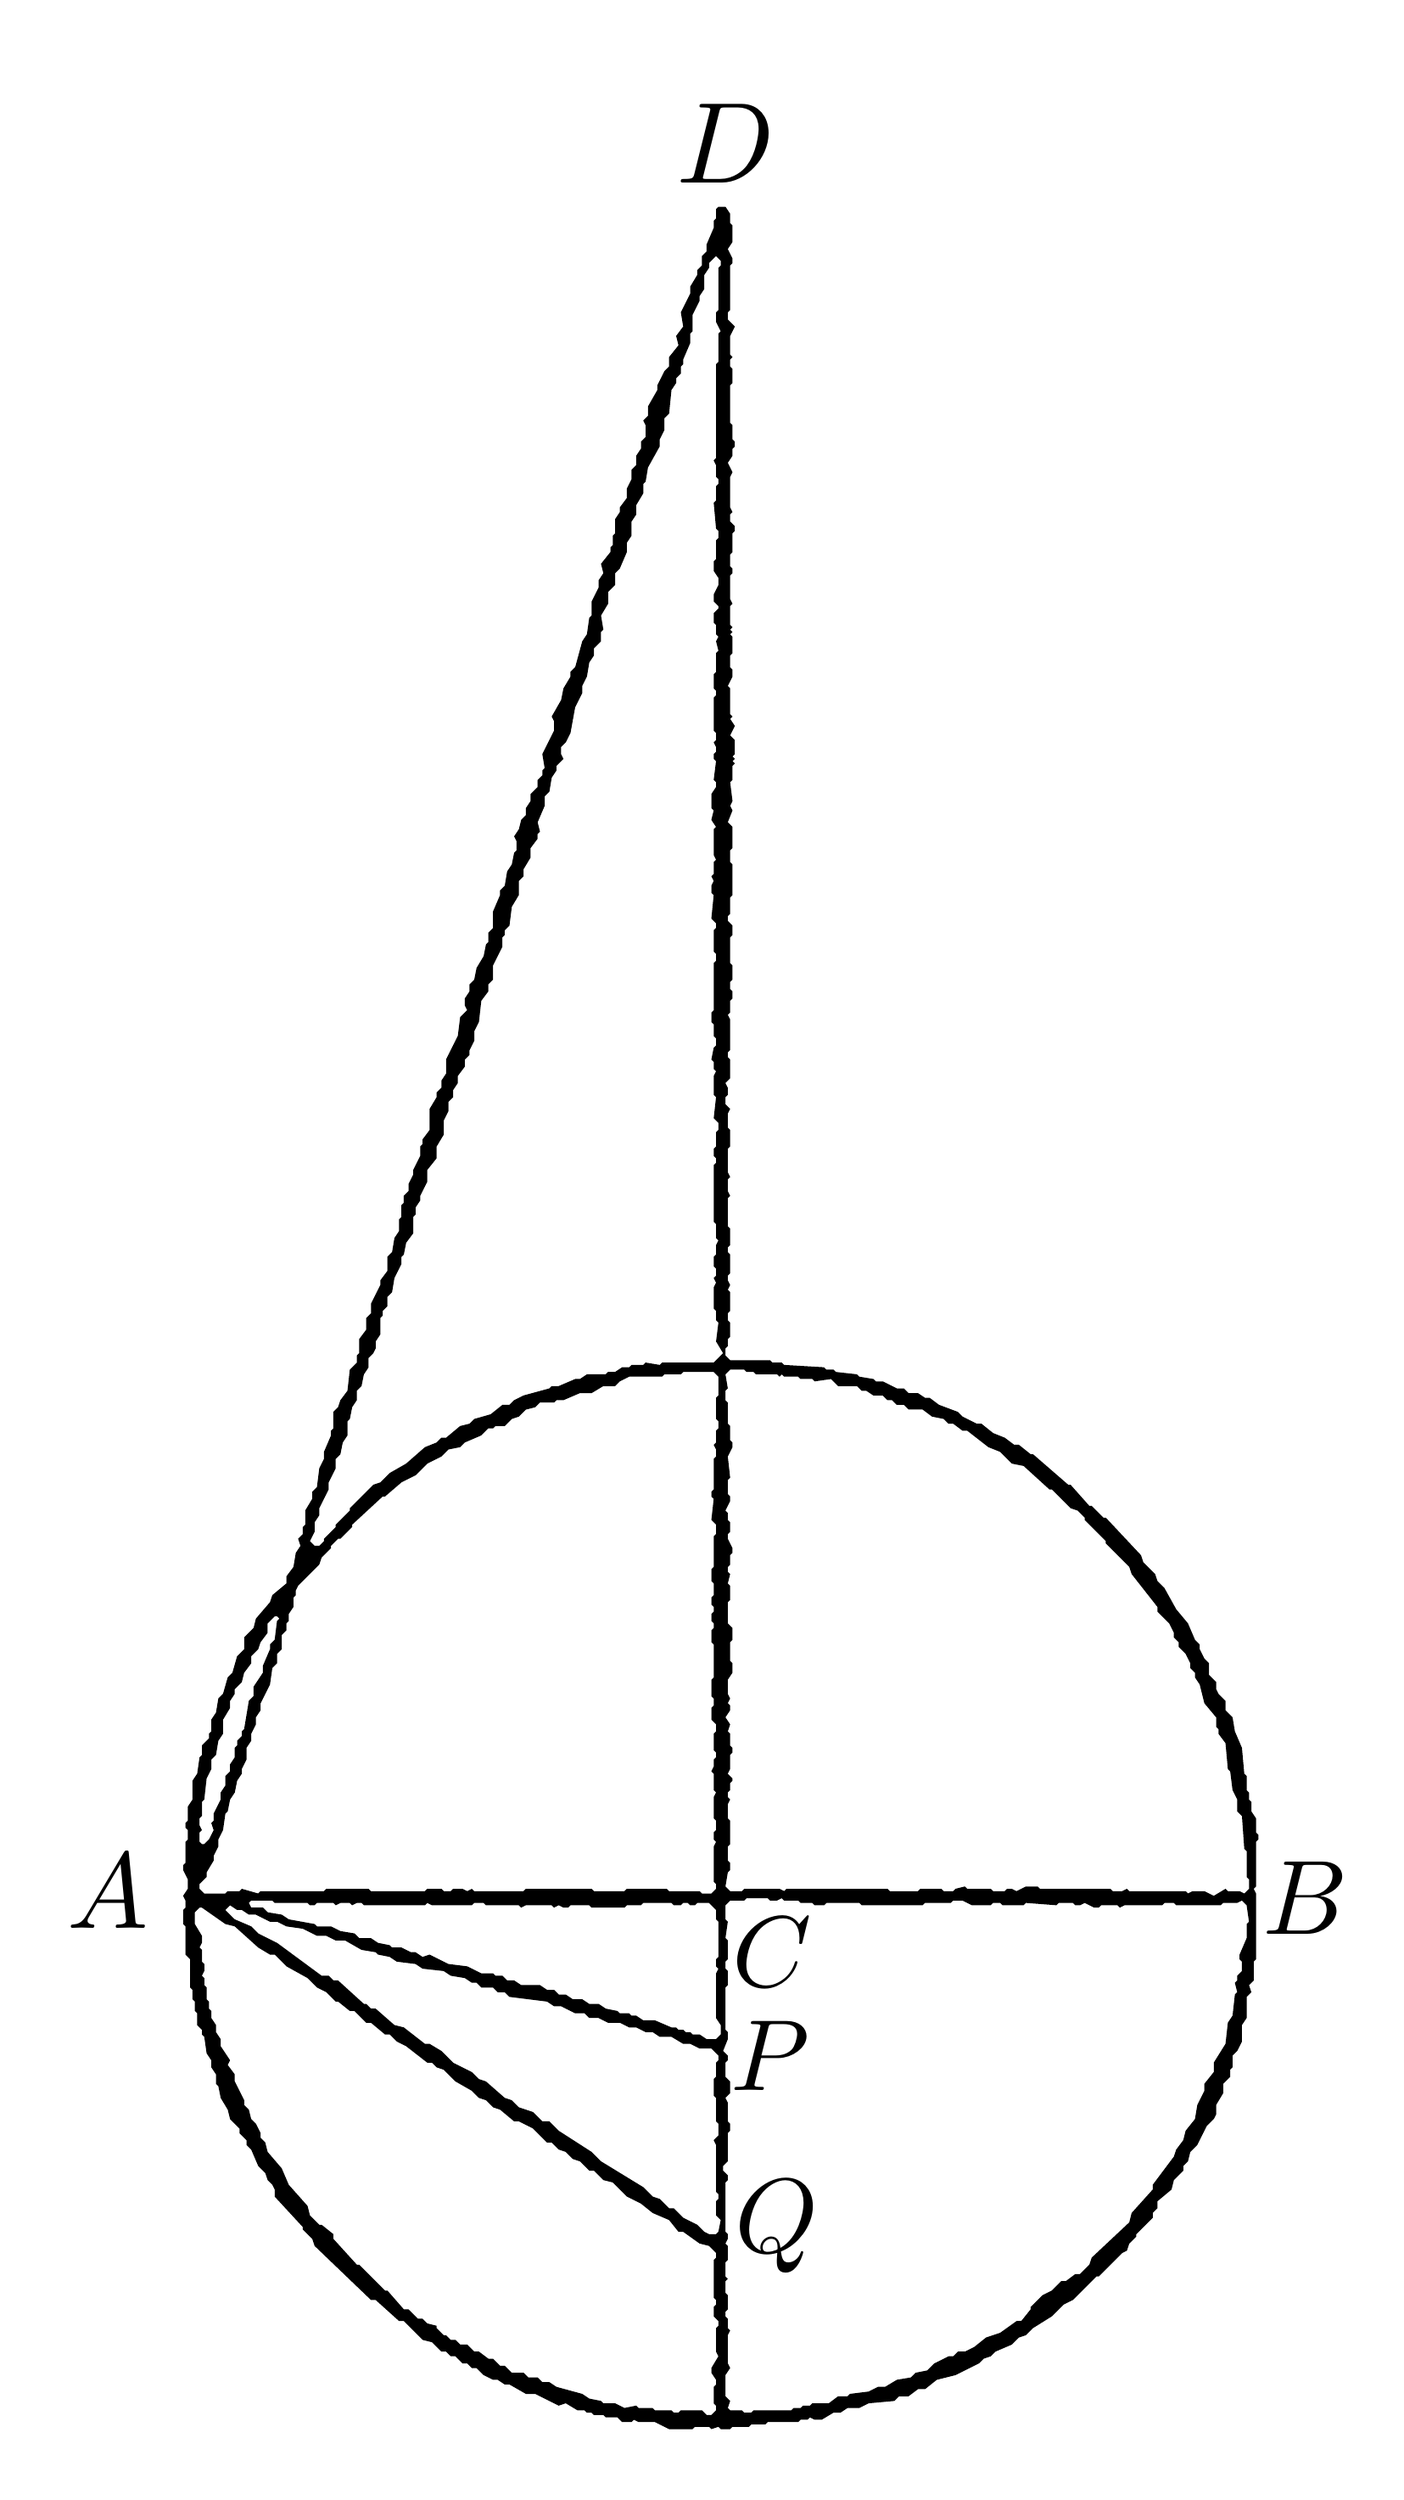
\begin{tikzpicture}[x=1pt,y=-1pt]
\path[use as bounding box] (0,0) rectangle (578,1044);
\path[fill=black,draw=none,even odd rule]
(299,78) -- (296,78) -- (295,79) -- (295,83) -- (294,84) -- (294,87) -- (291,94) -- (291,97) -- (289,99) -- (289,103) -- (287,105) -- (287,107) -- (284,112) -- (284,115) -- (280,123) -- (281,129) -- (278,133) -- (279,137) -- (275,142) -- (275,146) -- (273,148) -- (270,154) -- (270,156) -- (266,163) -- (266,167) -- (264,169) -- (265,171) -- (265,176) -- (263,178) -- (263,181) -- (261,184) -- (261,188) -- (259,190) -- (259,194) -- (257,198) -- (257,202) -- (254,206) -- (254,208) -- (252,211) -- (252,217) -- (251,218) -- (251,222) -- (250,223) -- (250,225) -- (246,230) -- (247,234) -- (245,237) -- (245,240) -- (242,246) -- (242,252) -- (241,253) -- (240,260) -- (238,263) -- (235,274) -- (233,276) -- (233,278) -- (230,283) -- (229,288) -- (225,295) -- (226,297) -- (226,301) -- (221,311) -- (222,317) -- (221,318) -- (221,320) -- (219,322) -- (219,325) -- (216,328) -- (216,331) -- (214,334) -- (214,337) -- (212,339) -- (211,343) -- (209,346) -- (210,348) -- (210,352) -- (209,353) -- (208,358) -- (206,361) -- (205,367) -- (203,369) -- (203,371) -- (200,378) -- (200,385) -- (198,387) -- (198,391) -- (197,392) -- (196,397) -- (193,402) -- (192,407) -- (190,409) -- (190,412) -- (188,415) -- (188,418) -- (189,420) -- (186,423) -- (185,431) -- (180,441) -- (180,447) -- (178,450) -- (178,453) -- (176,455) -- (176,457) -- (173,462) -- (173,471) -- (170,475) -- (170,477) -- (169,478) -- (169,482) -- (166,488) -- (166,490) -- (164,494) -- (164,497) -- (162,499) -- (162,502) -- (161,503) -- (161,508) -- (160,509) -- (160,514) -- (158,517) -- (157,523) -- (155,525) -- (155,531) -- (152,535) -- (152,537) -- (148,545) -- (148,549) -- (146,551) -- (146,556) -- (143,560) -- (143,566) -- (142,567) -- (142,570) -- (139,573) -- (138,582) -- (135,586) -- (134,589) -- (132,591) -- (132,598) -- (131,599) -- (131,601) -- (128,608) -- (128,611) -- (126,615) -- (125,623) -- (123,625) -- (123,628) -- (120,633) -- (120,639) -- (119,640) -- (119,643) -- (117,645) -- (118,648) -- (116,651) -- (115,657) -- (112,661) -- (112,664) -- (106,669) -- (105,672) -- (99,679) -- (98,683) -- (94,687) -- (94,692) -- (91,695) -- (89,702) -- (87,704) -- (85,711) -- (83,713) -- (82,719) -- (80,722) -- (80,727) -- (79,728) -- (79,730) -- (76,733) -- (76,737) -- (75,738) -- (74,745) -- (72,748) -- (72,756) -- (70,759) -- (70,765) -- (69,766) -- (69,768) -- (70,769) -- (70,773) -- (69,774) -- (69,783) -- (68,784) -- (68,786) -- (70,790) -- (70,794) -- (68,797) -- (69,799) -- (69,802) -- (68,803) -- (68,809) -- (69,810) -- (69,822) -- (71,824) -- (71,836) -- (72,837) -- (72,841) -- (73,842) -- (73,846) -- (74,847) -- (74,852) -- (76,854) -- (76,856) -- (77,857) -- (78,864) -- (80,867) -- (80,870) -- (82,873) -- (82,877) -- (83,878) -- (84,883) -- (87,888) -- (88,892) -- (92,896) -- (92,898) -- (95,901) -- (95,903) -- (97,905) -- (100,912) -- (103,915) -- (104,918) -- (106,920) -- (107,922) -- (107,925) -- (119,938) -- (119,939) -- (123,943) -- (124,946) -- (148,969) -- (150,969) -- (160,978) -- (162,978) -- (170,986) -- (174,987) -- (178,991) -- (180,991) -- (182,993) -- (184,993) -- (187,996) -- (189,996) -- (191,998) -- (193,998) -- (196,1001) -- (200,1003) -- (202,1003) -- (205,1005) -- (207,1005) -- (214,1009) -- (218,1009) -- (228,1014) -- (231,1013) -- (236,1016) -- (239,1016) -- (240,1017) -- (242,1017) -- (243,1018) -- (247,1018) -- (248,1019) -- (253,1019) -- (255,1021) -- (259,1021) -- (260,1020) -- (262,1021) -- (269,1021) -- (275,1024) -- (285,1024) -- (286,1023) -- (292,1023) -- (293,1024) -- (296,1023) -- (297,1024) -- (301,1024) -- (302,1023) -- (309,1023) -- (310,1022) -- (316,1022) -- (317,1021) -- (330,1021) -- (331,1020) -- (334,1020) -- (335,1019) -- (337,1020) -- (340,1020) -- (345,1017) -- (348,1017) -- (351,1015) -- (356,1015) -- (360,1013) -- (371,1012) -- (373,1010) -- (377,1010) -- (381,1007) -- (384,1007) -- (389,1003) -- (397,1001) -- (407,996) -- (409,994) -- (412,993) -- (414,991) -- (421,988) -- (424,985) -- (427,984) -- (430,981) -- (438,976) -- (443,971) -- (447,969) -- (457,959) -- (458,959) -- (468,949) -- (470,948) -- (471,945) -- (474,942) -- (474,941) -- (481,934) -- (481,932) -- (483,930) -- (483,927) -- (489,922) -- (490,918) -- (494,914) -- (494,912) -- (496,910) -- (497,906) -- (500,903) -- (504,895) -- (507,892) -- (508,890) -- (508,886) -- (511,881) -- (511,877) -- (514,874) -- (514,871) -- (515,870) -- (515,865) -- (517,863) -- (519,859) -- (519,852) -- (521,849) -- (521,840) -- (523,838) -- (522,835) -- (524,833) -- (524,825) -- (525,824) -- (525,796) -- (524,794) -- (525,793) -- (525,774) -- (526,773) -- (526,771) -- (525,770) -- (525,764) -- (523,761) -- (523,757) -- (522,756) -- (522,753) -- (521,752) -- (521,746) -- (520,745) -- (519,734) -- (516,727) -- (515,721) -- (512,718) -- (512,714) -- (509,711) -- (508,709) -- (508,706) -- (505,703) -- (505,698) -- (503,696) -- (501,692) -- (501,690) -- (499,688) -- (496,681) -- (491,675) -- (486,666) -- (483,663) -- (482,660) -- (477,655) -- (476,652) -- (461,636) -- (460,636) -- (455,631) -- (454,631) -- (446,622) -- (445,622) -- (430,609) -- (429,609) -- (424,605) -- (422,605) -- (418,602) -- (413,600) -- (408,596) -- (406,596) -- (400,593) -- (398,591) -- (390,588) -- (386,585) -- (384,585) -- (381,583) -- (377,583) -- (375,581) -- (372,581) -- (366,578) -- (363,578) -- (362,577) -- (356,576) -- (355,575) -- (346,574) -- (345,573) -- (342,573) -- (341,572) -- (324,571) -- (323,570) -- (319,570) -- (318,569) -- (301,569) -- (299,567) -- (299,564) -- (300,563) -- (300,560) -- (301,559) -- (301,553) -- (300,552) -- (300,549) -- (301,548) -- (301,540) -- (300,539) -- (301,537) -- (300,535) -- (300,533) -- (301,532) -- (301,524) -- (300,523) -- (300,521) -- (301,520) -- (301,513) -- (300,512) -- (300,500) -- (301,499) -- (300,497) -- (300,492) -- (301,491) -- (300,489) -- (300,479) -- (301,478) -- (301,471) -- (300,470) -- (300,464) -- (301,462) -- (299,460) -- (299,457) -- (300,456) -- (300,453) -- (299,451) -- (301,449) -- (301,441) -- (300,440) -- (300,438) -- (301,437) -- (301,424) -- (300,422) -- (301,421) -- (301,416) -- (302,415) -- (302,412) -- (301,411) -- (301,408) -- (302,407) -- (302,401) -- (301,400) -- (301,389) -- (302,388) -- (302,384) -- (300,382) -- (300,380) -- (301,379) -- (301,372) -- (302,371) -- (302,358) -- (301,357) -- (301,352) -- (302,351) -- (302,342) -- (300,340) -- (302,335) -- (301,333) -- (302,331) -- (301,323) -- (302,322) -- (302,316) -- (303,315) -- (302,314) -- (303,313) -- (302,312) -- (303,311) -- (303,305) -- (301,303) -- (303,299) -- (301,296) -- (302,295) -- (301,294) -- (301,283) -- (300,282) -- (302,278) -- (302,275) -- (301,274) -- (301,269) -- (302,268) -- (302,261) -- (301,260) -- (302,259) -- (301,258) -- (302,257) -- (301,256) -- (301,248) -- (302,247) -- (301,245) -- (301,235) -- (302,234) -- (302,232) -- (301,231) -- (301,226) -- (302,225) -- (302,217) -- (303,216) -- (303,214) -- (301,212) -- (301,209) -- (302,208) -- (301,206) -- (301,193) -- (302,191) -- (300,187) -- (302,184) -- (302,181) -- (303,180) -- (303,178) -- (302,177) -- (302,171) -- (301,170) -- (301,154) -- (302,153) -- (302,147) -- (301,146) -- (301,143) -- (302,142) -- (301,141) -- (301,133) -- (303,129) -- (300,126) -- (300,123) -- (301,122) -- (301,103) -- (302,102) -- (302,100) -- (300,96) -- (302,93) -- (302,86) -- (301,85) -- (301,81) -- cycle
(73,804) -- (75,802) -- (76,802) -- (86,809) -- (90,810) -- (100,819) -- (105,822) -- (107,822) -- (112,827) -- (121,832) -- (125,836) -- (129,838) -- (133,842) -- (134,842) -- (139,846) -- (141,846) -- (146,851) -- (148,851) -- (154,856) -- (156,856) -- (159,859) -- (163,861) -- (172,868) -- (174,868) -- (176,870) -- (179,871) -- (184,876) -- (191,880) -- (194,883) -- (197,884) -- (200,887) -- (203,888) -- (209,893) -- (211,893) -- (217,896) -- (223,902) -- (225,902) -- (228,905) -- (231,906) -- (234,909) -- (237,910) -- (241,914) -- (243,914) -- (247,918) -- (251,919) -- (257,925) -- (263,928) -- (268,932) -- (275,935) -- (279,940) -- (281,940) -- (288,945) -- (292,946) -- (295,949) -- (295,951) -- (294,952) -- (294,968) -- (295,969) -- (295,971) -- (294,972) -- (294,976) -- (296,978) -- (296,980) -- (295,981) -- (295,991) -- (296,993) -- (293,998) -- (293,1000) -- (295,1003) -- (295,1005) -- (294,1006) -- (294,1013) -- (295,1014) -- (295,1016) -- (293,1018) -- (291,1018) -- (289,1016) -- (280,1016) -- (279,1017) -- (277,1017) -- (276,1016) -- (269,1016) -- (268,1015) -- (262,1015) -- (261,1014) -- (256,1015) -- (252,1013) -- (247,1013) -- (246,1012) -- (241,1011) -- (238,1009) -- (227,1006) -- (224,1004) -- (221,1004) -- (219,1002) -- (215,1002) -- (213,1000) -- (208,1000) -- (205,997) -- (203,997) -- (200,994) -- (198,994) -- (194,991) -- (192,991) -- (189,988) -- (186,988) -- (184,986) -- (182,986) -- (180,984) -- (179,984) -- (176,981) -- (176,980) -- (172,979) -- (170,977) -- (168,977) -- (164,973) -- (162,973) -- (155,965) -- (154,965) -- (143,954) -- (142,954) -- (132,943) -- (132,941) -- (127,937) -- (126,937) -- (122,933) -- (121,929) -- (113,920) -- (110,913) -- (104,906) -- (103,902) -- (101,900) -- (101,898) -- (99,894) -- (97,892) -- (96,888) -- (94,886) -- (94,884) -- (90,876) -- (90,873) -- (87,869) -- (88,867) -- (84,861) -- (84,858) -- (82,855) -- (82,852) -- (80,849) -- (80,846) -- (79,845) -- (79,842) -- (78,841) -- (78,836) -- (77,835) -- (77,832) -- (76,831) -- (77,829) -- (77,826) -- (76,825) -- (76,820) -- (75,819) -- (76,817) -- (76,814) -- (73,809) -- cycle
(86,803) -- (88,801) -- (91,803) -- (93,803) -- (96,805) -- (99,805) -- (105,808) -- (108,808) -- (112,810) -- (119,811) -- (125,814) -- (129,814) -- (133,816) -- (137,816) -- (144,820) -- (150,821) -- (151,822) -- (156,823) -- (159,825) -- (167,826) -- (170,828) -- (179,829) -- (182,831) -- (188,832) -- (191,834) -- (193,834) -- (195,836) -- (200,836) -- (202,838) -- (205,838) -- (207,840) -- (223,842) -- (226,844) -- (229,844) -- (235,847) -- (239,847) -- (241,849) -- (245,849) -- (249,851) -- (254,851) -- (258,853) -- (261,853) -- (265,855) -- (268,855) -- (271,857) -- (276,857) -- (281,860) -- (284,860) -- (288,862) -- (293,862) -- (296,865) -- (296,867) -- (295,868) -- (295,874) -- (294,875) -- (294,882) -- (295,883) -- (295,893) -- (296,894) -- (296,899) -- (294,901) -- (295,903) -- (295,923) -- (296,924) -- (296,926) -- (295,927) -- (295,933) -- (297,935) -- (296,940) -- (295,941) -- (292,941) -- (290,940) -- (287,937) -- (281,934) -- (277,930) -- (275,930) -- (271,926) -- (268,925) -- (264,921) -- (246,910) -- (242,906) -- (228,897) -- (224,893) -- (221,893) -- (217,889) -- (211,887) -- (208,884) -- (205,883) -- (197,876) -- (194,875) -- (191,872) -- (183,868) -- (178,863) -- (173,860) -- (171,860) -- (162,853) -- (158,852) -- (150,845) -- (148,845) -- (146,843) -- (145,843) -- (134,833) -- (132,833) -- (130,831) -- (127,831) -- (108,817) -- (100,813) -- (97,810) -- (90,807) -- cycle
(96,800) -- (97,799) -- (106,799) -- (107,800) -- (121,800) -- (122,801) -- (124,801) -- (125,800) -- (132,800) -- (133,801) -- (135,800) -- (139,800) -- (140,801) -- (142,800) -- (144,800) -- (145,801) -- (171,801) -- (172,800) -- (174,801) -- (191,801) -- (192,800) -- (196,800) -- (197,801) -- (211,801) -- (212,802) -- (214,801) -- (225,801) -- (226,802) -- (228,801) -- (230,802) -- (232,802) -- (233,801) -- (241,801) -- (242,802) -- (256,802) -- (257,801) -- (263,801) -- (264,800) -- (276,800) -- (277,801) -- (280,801) -- (281,800) -- (283,800) -- (284,801) -- (286,801) -- (287,800) -- (292,800) -- (295,803) -- (295,807) -- (296,808) -- (296,823) -- (295,824) -- (295,827) -- (296,828) -- (295,830) -- (295,849) -- (297,852) -- (297,856) -- (295,858) -- (291,858) -- (288,856) -- (285,856) -- (284,855) -- (282,855) -- (281,854) -- (279,854) -- (278,853) -- (276,853) -- (269,850) -- (264,850) -- (261,848) -- (259,848) -- (258,847) -- (254,847) -- (253,846) -- (248,845) -- (245,843) -- (241,843) -- (238,841) -- (234,841) -- (231,839) -- (228,839) -- (226,837) -- (223,837) -- (220,835) -- (212,835) -- (209,833) -- (206,833) -- (204,831) -- (201,831) -- (200,830) -- (195,830) -- (189,827) -- (181,826) -- (173,822) -- (170,823) -- (167,821) -- (165,821) -- (161,819) -- (157,819) -- (156,818) -- (151,817) -- (148,815) -- (143,815) -- (141,813) -- (135,812) -- (131,810) -- (125,810) -- (124,809) -- (113,807) -- (110,805) -- (104,804) -- (102,802) -- (97,802) -- cycle
(519,799) -- (521,801) -- (522,808) -- (521,809) -- (521,815) -- (518,822) -- (518,824) -- (519,825) -- (519,829) -- (517,831) -- (517,833) -- (516,834) -- (517,838) -- (516,839) -- (515,848) -- (513,851) -- (512,860) -- (507,868) -- (507,872) -- (503,877) -- (503,880) -- (500,886) -- (499,892) -- (495,897) -- (494,901) -- (491,905) -- (490,908) -- (481,920) -- (481,922) -- (472,932) -- (471,936) -- (455,951) -- (454,954) -- (450,958) -- (448,958) -- (444,961) -- (442,961) -- (438,965) -- (434,967) -- (429,972) -- (429,973) -- (425,978) -- (423,978) -- (416,983) -- (410,985) -- (405,989) -- (401,991) -- (398,991) -- (396,993) -- (394,993) -- (388,996) -- (385,999) -- (380,1000) -- (378,1002) -- (372,1003) -- (367,1006) -- (364,1006) -- (360,1008) -- (352,1009) -- (351,1010) -- (347,1010) -- (343,1013) -- (336,1013) -- (335,1014) -- (332,1014) -- (331,1015) -- (328,1015) -- (327,1016) -- (311,1016) -- (310,1017) -- (307,1017) -- (306,1016) -- (301,1016) -- (300,1015) -- (301,1012) -- (299,1010) -- (299,1001) -- (301,998) -- (300,996) -- (300,984) -- (301,982) -- (300,981) -- (300,977) -- (299,976) -- (299,974) -- (300,973) -- (300,967) -- (299,966) -- (299,961) -- (300,960) -- (299,959) -- (299,953) -- (300,952) -- (300,946) -- (299,945) -- (300,943) -- (300,941) -- (299,940) -- (299,919) -- (300,918) -- (300,916) -- (298,914) -- (298,912) -- (300,910) -- (300,898) -- (301,897) -- (301,894) -- (300,893) -- (300,885) -- (299,883) -- (301,881) -- (301,876) -- (299,874) -- (299,868) -- (300,867) -- (300,865) -- (298,863) -- (300,858) -- (300,855) -- (299,854) -- (299,836) -- (300,835) -- (300,829) -- (299,828) -- (299,825) -- (300,824) -- (300,816) -- (299,815) -- (300,808) -- (299,807) -- (299,801) -- (301,799) -- (307,799) -- (308,798) -- (317,798) -- (318,799) -- (321,799) -- (323,798) -- (324,799) -- (330,799) -- (331,800) -- (336,800) -- (337,801) -- (341,801) -- (342,800) -- (356,800) -- (357,801) -- (383,801) -- (384,800) -- (395,800) -- (396,799) -- (400,799) -- (404,801) -- (412,801) -- (413,800) -- (416,800) -- (417,801) -- (426,801) -- (427,800) -- (440,801) -- (441,800) -- (447,800) -- (448,801) -- (450,801) -- (452,800) -- (456,802) -- (458,802) -- (459,801) -- (466,801) -- (467,802) -- (469,801) -- (485,801) -- (486,800) -- (490,800) -- (491,801) -- (510,801) -- (511,800) -- (517,800) -- cycle
(108,678) -- (109,679) -- (108,680) -- (107,688) -- (105,690) -- (105,692) -- (102,699) -- (102,702) -- (98,708) -- (98,712) -- (96,714) -- (94,726) -- (93,727) -- (93,729) -- (91,731) -- (91,733) -- (90,734) -- (90,738) -- (88,741) -- (88,744) -- (86,746) -- (86,750) -- (84,753) -- (84,756) -- (81,762) -- (81,765) -- (80,766) -- (81,769) -- (79,773) -- (77,775) -- (76,775) -- (75,774) -- (75,770) -- (76,769) -- (75,767) -- (75,764) -- (76,763) -- (76,757) -- (77,756) -- (78,747) -- (80,743) -- (80,739) -- (82,737) -- (83,731) -- (85,728) -- (85,722) -- (88,717) -- (88,714) -- (90,711) -- (90,709) -- (93,706) -- (94,702) -- (97,698) -- (97,695) -- (100,692) -- (101,689) -- (104,685) -- (104,681) -- (107,678) -- cycle
(294,574) -- (296,576) -- (296,584) -- (295,585) -- (295,594) -- (296,595) -- (296,598) -- (295,599) -- (295,604) -- (294,605) -- (295,607) -- (295,610) -- (294,611) -- (294,624) -- (293,625) -- (293,627) -- (294,628) -- (293,637) -- (295,639) -- (295,643) -- (294,644) -- (294,657) -- (293,658) -- (293,663) -- (294,664) -- (294,669) -- (293,670) -- (293,673) -- (294,674) -- (294,676) -- (293,677) -- (293,680) -- (294,681) -- (294,683) -- (293,684) -- (293,689) -- (294,690) -- (294,704) -- (293,705) -- (293,712) -- (294,713) -- (294,716) -- (293,717) -- (293,722) -- (295,724) -- (295,727) -- (294,728) -- (294,735) -- (295,736) -- (295,738) -- (294,739) -- (294,742) -- (293,744) -- (294,745) -- (294,752) -- (295,753) -- (294,755) -- (294,764) -- (295,765) -- (295,769) -- (294,770) -- (294,773) -- (295,774) -- (294,776) -- (294,791) -- (295,792) -- (295,794) -- (293,796) -- (289,796) -- (288,795) -- (275,795) -- (274,794) -- (257,794) -- (256,795) -- (243,795) -- (242,794) -- (214,794) -- (213,795) -- (192,795) -- (191,794) -- (189,795) -- (187,794) -- (183,794) -- (182,795) -- (179,795) -- (178,794) -- (172,794) -- (171,795) -- (148,795) -- (147,794) -- (129,794) -- (128,795) -- (101,795) -- (100,796) -- (93,794) -- (92,795) -- (87,795) -- (86,796) -- (77,796) -- (75,794) -- (75,792) -- (78,789) -- (78,787) -- (81,782) -- (81,780) -- (83,776) -- (83,773) -- (85,769) -- (86,762) -- (87,761) -- (88,756) -- (90,753) -- (91,748) -- (93,745) -- (93,743) -- (95,739) -- (95,734) -- (97,731) -- (97,728) -- (99,724) -- (99,721) -- (101,718) -- (101,715) -- (105,707) -- (106,700) -- (108,698) -- (108,694) -- (110,692) -- (110,686) -- (112,684) -- (112,681) -- (113,680) -- (113,677) -- (115,674) -- (115,670) -- (116,669) -- (116,667) -- (117,665) -- (126,656) -- (127,653) -- (131,649) -- (131,648) -- (134,645) -- (135,645) -- (140,640) -- (140,639) -- (153,627) -- (154,627) -- (161,621) -- (167,618) -- (172,613) -- (178,610) -- (181,607) -- (186,606) -- (188,604) -- (195,601) -- (198,598) -- (200,598) -- (201,597) -- (205,597) -- (208,594) -- (211,593) -- (214,590) -- (218,589) -- (220,587) -- (226,587) -- (227,586) -- (230,586) -- (237,583) -- (242,583) -- (247,580) -- (252,580) -- (254,578) -- (258,576) -- (272,576) -- (273,575) -- (280,575) -- (281,574) -- cycle
(301,573) -- (307,573) -- (308,574) -- (311,574) -- (312,575) -- (321,575) -- (322,576) -- (323,575) -- (324,576) -- (330,576) -- (331,577) -- (336,577) -- (337,578) -- (344,577) -- (347,580) -- (355,580) -- (357,582) -- (359,582) -- (362,584) -- (366,584) -- (368,586) -- (370,586) -- (372,588) -- (375,588) -- (377,590) -- (383,590) -- (387,593) -- (392,594) -- (394,596) -- (396,596) -- (400,599) -- (402,599) -- (411,606) -- (416,608) -- (421,613) -- (426,614) -- (437,624) -- (438,624) -- (446,632) -- (449,633) -- (452,636) -- (452,637) -- (461,646) -- (461,647) -- (471,657) -- (472,660) -- (483,674) -- (483,676) -- (488,681) -- (490,685) -- (490,687) -- (492,689) -- (492,691) -- (495,694) -- (497,698) -- (497,700) -- (499,702) -- (499,704) -- (501,707) -- (503,715) -- (508,721) -- (508,725) -- (509,726) -- (509,728) -- (512,732) -- (513,743) -- (514,744) -- (515,752) -- (517,756) -- (517,761) -- (519,763) -- (520,777) -- (521,778) -- (521,789) -- (522,790) -- (522,794) -- (520,796) -- (518,795) -- (513,795) -- (512,794) -- (507,797) -- (503,795) -- (498,795) -- (496,796) -- (495,795) -- (471,795) -- (470,794) -- (468,795) -- (464,795) -- (463,794) -- (433,794) -- (432,793) -- (427,793) -- (423,795) -- (421,794) -- (419,794) -- (418,795) -- (413,795) -- (412,794) -- (402,794) -- (401,793) -- (397,794) -- (396,795) -- (392,795) -- (391,794) -- (382,794) -- (381,795) -- (369,795) -- (368,794) -- (325,794) -- (324,795) -- (322,794) -- (307,794) -- (306,795) -- (301,795) -- (299,793) -- (300,787) -- (301,786) -- (301,783) -- (300,782) -- (300,776) -- (301,775) -- (301,765) -- (300,764) -- (300,758) -- (301,756) -- (300,755) -- (300,753) -- (301,752) -- (301,749) -- (302,748) -- (302,747) -- (300,745) -- (301,743) -- (301,737) -- (302,736) -- (302,734) -- (301,733) -- (301,728) -- (300,727) -- (301,724) -- (299,721) -- (301,718) -- (301,716) -- (300,715) -- (301,713) -- (300,711) -- (300,705) -- (302,702) -- (302,698) -- (301,697) -- (301,689) -- (302,688) -- (302,683) -- (300,681) -- (300,672) -- (301,671) -- (301,665) -- (300,664) -- (301,660) -- (300,659) -- (300,657) -- (301,656) -- (301,652) -- (302,651) -- (302,649) -- (300,645) -- (300,643) -- (301,642) -- (301,638) -- (300,637) -- (300,634) -- (299,633) -- (301,629) -- (301,627) -- (300,626) -- (300,620) -- (301,619) -- (300,610) -- (302,606) -- (302,604) -- (301,603) -- (301,597) -- (300,596) -- (300,587) -- (299,586) -- (299,582) -- (300,581) -- (299,575) -- cycle
(295,99) -- (297,101) -- (297,103) -- (296,104) -- (296,122) -- (295,123) -- (295,127) -- (297,131) -- (296,132) -- (296,144) -- (295,145) -- (295,185) -- (294,186) -- (295,188) -- (295,193) -- (296,194) -- (296,196) -- (295,197) -- (295,203) -- (294,204) -- (295,215) -- (296,216) -- (296,219) -- (295,220) -- (295,228) -- (294,229) -- (294,233) -- (296,236) -- (296,239) -- (294,243) -- (294,246) -- (296,248) -- (296,249) -- (294,251) -- (294,255) -- (295,256) -- (295,260) -- (296,261) -- (295,263) -- (296,267) -- (295,268) -- (295,276) -- (294,277) -- (294,283) -- (295,284) -- (295,286) -- (294,287) -- (294,301) -- (295,302) -- (295,305) -- (294,306) -- (295,308) -- (295,310) -- (294,311) -- (294,313) -- (295,314) -- (294,322) -- (295,323) -- (295,325) -- (293,328) -- (293,334) -- (294,335) -- (293,339) -- (295,342) -- (294,343) -- (294,354) -- (295,356) -- (294,357) -- (294,362) -- (293,363) -- (294,365) -- (293,367) -- (293,370) -- (294,371) -- (293,381) -- (295,383) -- (295,385) -- (294,386) -- (294,395) -- (295,396) -- (295,399) -- (294,400) -- (294,420) -- (293,421) -- (293,425) -- (294,426) -- (294,431) -- (295,432) -- (295,435) -- (294,436) -- (293,441) -- (294,442) -- (294,445) -- (295,446) -- (294,448) -- (294,456) -- (295,457) -- (294,466) -- (296,468) -- (296,471) -- (295,472) -- (295,478) -- (294,479) -- (294,482) -- (295,483) -- (295,485) -- (294,486) -- (294,510) -- (295,511) -- (295,517) -- (296,518) -- (295,520) -- (295,524) -- (294,525) -- (294,529) -- (295,530) -- (295,533) -- (294,534) -- (295,536) -- (294,538) -- (294,547) -- (295,548) -- (295,552) -- (296,553) -- (295,561) -- (298,566) -- (294,570) -- (272,570) -- (271,571) -- (265,570) -- (264,571) -- (259,571) -- (258,572) -- (255,572) -- (252,574) -- (249,574) -- (248,575) -- (240,575) -- (237,577) -- (235,577) -- (228,580) -- (225,580) -- (224,581) -- (213,584) -- (209,586) -- (207,588) -- (204,588) -- (199,592) -- (192,594) -- (190,596) -- (186,597) -- (180,602) -- (178,602) -- (176,604) -- (171,606) -- (163,613) -- (156,617) -- (152,621) -- (149,622) -- (139,632) -- (139,633) -- (133,639) -- (133,640) -- (128,645) -- (128,646) -- (126,648) -- (124,648) -- (122,646) -- (124,642) -- (124,638) -- (126,635) -- (126,632) -- (130,624) -- (130,621) -- (133,615) -- (133,611) -- (135,609) -- (136,604) -- (138,601) -- (138,595) -- (139,594) -- (140,589) -- (142,586) -- (142,582) -- (144,580) -- (145,575) -- (147,572) -- (147,568) -- (149,566) -- (150,564) -- (150,561) -- (152,558) -- (152,551) -- (153,550) -- (153,548) -- (155,546) -- (155,542) -- (157,540) -- (158,534) -- (161,528) -- (161,525) -- (162,524) -- (163,519) -- (166,515) -- (166,508) -- (167,507) -- (167,504) -- (169,501) -- (169,499) -- (172,493) -- (172,488) -- (176,483) -- (176,478) -- (179,473) -- (179,467) -- (181,463) -- (181,459) -- (183,457) -- (183,454) -- (185,451) -- (185,448) -- (188,444) -- (188,441) -- (190,439) -- (190,437) -- (192,433) -- (192,429) -- (194,425) -- (195,416) -- (198,412) -- (198,409) -- (200,407) -- (200,401) -- (204,393) -- (204,389) -- (205,388) -- (205,386) -- (207,384) -- (208,376) -- (211,371) -- (211,365) -- (213,363) -- (213,360) -- (216,355) -- (216,351) -- (219,347) -- (219,345) -- (220,344) -- (219,340) -- (222,333) -- (222,329) -- (224,327) -- (225,321) -- (227,318) -- (227,316) -- (230,313) -- (229,311) -- (229,308) -- (231,306) -- (233,302) -- (235,291) -- (238,285) -- (238,282) -- (240,278) -- (241,272) -- (243,269) -- (243,266) -- (246,263) -- (246,259) -- (247,258) -- (246,252) -- (249,247) -- (249,242) -- (252,239) -- (252,234) -- (254,232) -- (257,225) -- (257,221) -- (259,218) -- (259,212) -- (261,209) -- (261,205) -- (264,200) -- (264,196) -- (265,195) -- (266,189) -- (271,180) -- (271,177) -- (273,173) -- (273,168) -- (275,166) -- (276,156) -- (278,153) -- (278,151) -- (280,149) -- (280,146) -- (281,145) -- (281,143) -- (284,136) -- (284,132) -- (285,131) -- (285,124) -- (288,118) -- (288,116) -- (290,113) -- (290,107) -- (292,104) -- (292,102) -- cycle;
\node[inner sep=0pt,font=\fontsize{10}{10}\selectfont] at (299,51) {\scalebox{4.9}{$D$}};
\node[inner sep=0pt,font=\fontsize{10}{10}\selectfont] at (36,795) {\scalebox{4.6}{$A$}};
\node[inner sep=0pt,font=\fontsize{10}{10}\selectfont] at (546,798) {\scalebox{4.5}{$B$}};
\node[inner sep=0pt,font=\fontsize{10}{10}\selectfont] at (319,821) {\scalebox{4.3}{$C$}};
\node[inner sep=0pt,font=\fontsize{10}{10}\selectfont] at (318,865) {\scalebox{4.3}{$P$}};
\node[inner sep=0pt,font=\fontsize{10}{10}\selectfont] at (321,938) {\scalebox{4.5}{$Q$}};
\end{tikzpicture}%
}
\end{center}
\indent $P$ und $Q$ Darstellung eines und desselben Punkts der Kugel in den beiden Projectionen; $ACB$ gegen $CPQ$ normal, Winkel $CAP = PAQ$.

$AD$ normal gegen $PA$ und $D$ auf der verlängerten $QPC$, wird $D$ die stereographische Darstellung des jenem Kugelpunkte gegenüberliegenden.

Ein Kreis um den Mittelpunkt $Q$ mit dem Radius $QA$ ist die stereographische Darstellung desjenigen grössten Kreises, der jenen Kugelpunkt zum Pole hat.

Ist $a+bi$ die complexe Zahl für centrale Projection, $r$ Halbmesser, so ist die complexe Zahl für die stereographische Projection

\[
\frac{(a+ib)r}{aa+bb}\left\{\BareRoot{(aa+bb+rr)}-r\right\}.
\]


